\documentclass[12pt,a4paper]{article}

\usepackage[utf8]{inputenc}
\usepackage[T1]{fontenc}
\usepackage[french]{babel}

\usepackage{amsmath, amssymb}

\usepackage{graphicx}
\usepackage{caption}

\usepackage{siunitx} % Pour les unités

\usepackage{geometry}
\geometry{top=2cm, bottom=2.5cm, left=3cm, right=3cm}
\setlength{\parindent}{0pt}

\usepackage[sfdefault]{roboto}

\usepackage{enumitem}

\usepackage{hyperref}

\usepackage{xcolor}

\usepackage{multicol}
\setlength{\columnseprule}{1pt}
\def\columnseprulecolor{\color{gray}}




\usepackage{tcolorbox}

\usepackage{wrapfig}

\usepackage{float}

\usepackage{tikz}



















\title{Ouvrages spéciaux : TD 1 passrelle en BA}
\author{}
\date{\today}

\begin{document}
	
	
	
	\maketitle
	
	\tableofcontents
	
	\newpage
	
	
	\part{TD 01}
	
	
	
	\section{Determination des armatures de la passerelle en BA}
	
	Cela ce fait a l'ELU.
	
	
	\subsection{Armature de la dalle}
	
	le calcul se fait a 1m de dalle.
	
	\subsubsection{Evaluation des charges}
	
	\begin{itemize}
		\item Revetement $\rightarrow 1000 ~\unit{N\per m^{2}} $
		\item Poids de la dalle $\rightarrow 1 \cdot 0,08 \cdot 25000 = 2000 ~\unit{N\per m^{2}} $ 
		\item Revetement + poids de la dalle = $ g = 3000 ~\unit{N\per m^{2}} $ 
	\end{itemize}
	
	\[ P_{ELU}  =  1,35 \cdot g  +  1,5 \cdot q  = 1,35 \cdot 3000  + 1,5 \cdot 4000  = 10050 ~\unit{N\per m^{2}} \]
	
	\vspace{\baselineskip}
	
	\subsubsection{Calcul des armature}
	
	Le moment maximale pour la dalle reposant sur deux appuis a pour valeur en considérant une largeur de 1m et compte et compte tenu des coefficients de majoration : 
	
	\[ M_{0}  =  \dfrac{P_{ELU} \cdot l^{2}}{8}  =  \dfrac{10050 \cdot 2^{2}}{8}  =  5025 ~\unit{Nm} \]
	
	La dalle etant semi encastrée sur les poutres latérales, nous aurons : 
	
	\begin{itemize}
		\item Sur appuis : $ M_{R}  =  0,4 \cdot M_{0} = 2010 ~\unit{Nm} $
		\item En travée : $ M_{t} = 0,85 \cdot M_{0} = 4271,25 ~\unit{Nm} $
	\end{itemize}
	
	\vspace{\baselineskip}
	
	\[ FeE400 \rightarrow \mu_{l}  = 0,392 \]
	
	
	\vspace{\baselineskip}
	
	\subsubsection{section d'armature en travée}
	
	Pour la section en travée nous avons :
	
	\begin{itemize}
		\item Fissuration préjudiciable donc enrobage de la dalle est de $ c  =  2,5 ~\unit{cm} $
		\item La hauteur utile $ \rightarrow d = h - c = 8 - 2,5 = 5,5 ~\unit{cm} $
	\end{itemize}
	
	
	\[ \mu  = \dfrac{M^{\max}_{travée}}{b \cdot d^{2} \cdot f_{bu}}  = \dfrac{4271,25 \cdot 10^{2}}{100 \cdot 5,5^{2} \cdot 14,2 \cdot 10^{2}}  = 0,099 \]
	
	\[ \mu  = 0,099 < \mu_{l}  = 0,392 \]
	
	Donc section simplement armé $ A_{sc}  = 0 $
	
	\[ A_{st}  = \dfrac{M^{\max}_{travée}}{\beta \cdot d \cdot \sigma_{st}} \]
	
	Depuis les tableaux on a $ \mu  =  0,099 \rightarrow \beta = 0,9478 $
	
	\[ A_{st}  =  \dfrac{4271,25 \cdot 10^{2}}{0,9478 \cdot 5,5 \cdot \dfrac{400}{1,15} \cdot 10^{2}} \]
	
	\[ A_{st}  =  2,357 ~\unit{cm^{2}} \]
	
	\vspace{\baselineskip}
	
	\subsubsection{Section d'armature en appuie}
	
	\[ \mu = \dfrac{M_{appuie}^{\max}}{b \cdot d^{2} \cdot f_{bu}}
	= \dfrac{2010 \cdot 10^{2}}{100 \cdot 5,5^{2} \cdot 14,2 \cdot 10^{2}} \]
	
	
	\[\rightarrow \mu  = 0,0467 < \mu_{l}  = 0,392 \rightarrow \text{section simplement armé } A_{sc} = 0 \]
	
	Depuis les tableau on a pas une valeur correspondate a $ \beta $ avec $ \mu  = 0,0467 $ donc on doit interpolé.
	
	\[ \mu_{1}  = 0,046 \rightarrow \beta_{1}  = 0,9764 \]
	
	\[ \mu_{2}  = 0,047 \rightarrow \beta_{2} = 0,9759 \]
	
	\[ \beta_{i}  = \beta_{1} + (\beta_{2} - \beta_{1}) \cdot \dfrac{\mu_{i} - \mu_{1}}{\mu_{2} - \mu_{1}}
	= 0,9764  + (0,9759 - 9764) \cdot \dfrac{0,0467 - 0,046}{0,047 - 0,046}  = 0,97605
	\]
	
	\[ A_{st}  =  \dfrac{M_{app}^{\max}}{\beta \cdot d \cdot \sigma_{st}}  = \dfrac{2010 \cdot 10^{2}}{0,97605 \cdot 5,5 \cdot 348 \cdot 10^{2}} \]
	
	\[ \rightarrow A_{st}  = 1,076 ~\unit{cm^{2}} \]
	
	\subsubsection{Vérification de la condition de non fragilité CNF}
	
	La section des armatures longitudinales doit vérifier la condition suivante : 
	
	\[ A_{adopté} > A_{\min} = \dfrac{0,23 \cdot b \cdot d \cdot f_{t28}}{fe} \]
	
	\[ A_{\min}  = \dfrac{0,23 \cdot 100 \cdot 5,5 \cdot 2,1}{400} = 0,664 ~\unit{cm^{2}} \]
	
	\[ A_{adopté} > A_{\min} \text{ Condition vérifier} \]
	
	
	
	\subsubsection{Effort tranchant max sur appuie}
	
	\[ V_{\max}  = P_{ELU} \cdot \dfrac{l}{2}  = 10050 \cdot \dfrac{2}{2} = 10050 ~\unit{N} \]
	
	\paragraph{Contrainte tangentielle max} :
	
	On doit vérifier que : \[ \tau_{u} = \dfrac{V_{\max}}{b_{0} \cdot d} \leq \overline{\tau}_{u} \]
	
	avec $ b_{0} = b $ section rectangulaire.
	
	\[ \overline{\tau}_{u}  =  \min \bigg\{ 0,05 \cdot f_{c28} \quad;\quad 5 ~\unit{MPa} \bigg\} \rightarrow \overline{\tau}_{u}  = 1,25 ~\unit{MPa} \]
	
	\[ \tau = \dfrac{V_{u}}{b \cdot d} = \dfrac{10050}{1000 ~\unit{mm} \cdot 55 ~\unit{mm}}  = 0,183 ~\unit{MPa} \]
	
	\[ \tau < \overline{\tau}_{u} \text{condition vérifiée} \]
	
	On doit voir si des vérification des armatures sont nécissaire en zone d'about(appuie)
	
	\[ V_{\max} + \dfrac{M_{u}}{0,9 \cdot d} = 10050 + \dfrac{ - 201000}{0,9 \cdot 5,5} =  - 30556,06 < 0 \]
	
	Donc aucune vérification des armatures est nécissaire.
	
	
	
	\subsection{Armatures de la poutre}
	
	\subsubsection{Evaluation des charges}
	
	\begin{itemize}
		\item Garde du corp : $ 1,35 \cdot \dfrac{800}{2}  = 540 ~\unit{N\per ml} $
		\item Poids propre de la poutre pour 1ml : $ 1,35 \cdot 0,8 \cdot 0,25 \cdot 1 \cdot 25000  = 6750 $
		\item Reaction de l'hourdis : $ 10050 ~\unit{N \per ml} $
	\end{itemize}
	
	\[ P_{ELU}  = 540  + 6750 + 10050  = 17340 ~\unit{N\per ml} \]
	
	
	\subsubsection{Calcul en travée}
	
	Moment maximale en travée
	
	\[ M_{0} = \dfrac{P_{ELU} \cdot l^{2}}{8}  = \dfrac{17340 \cdot 12^{2}}{8} = 312120 ~\unit{Nm} \]
	
	nous avons $ d = 74 ~\unit{cm} $
	
	\[ \mu = \dfrac{M_{t}^{\max}}{b \cdot d^{2} \cdot f_{bu}} = \dfrac{312120 \cdot 10^{2}}{25 \cdot 74^{2} \cdot 14,2 \cdot 10^{2}} = 0,1605 \]
	
	\[ \mu = 0,1605 < \mu_{l} = 0,392 \] 
	
	Section simplement armé $ A_{sc} = 0 $
	
	avec interpolation on aura $ \beta  = 0,912 $
	
	\[ A_{st} = \dfrac{M_{t}^{\max}}{\beta \cdot d \cdot \sigma_{st}} = \dfrac{312120 \cdot 10^{2}}{0,912 \cdot 74 \cdot 348 \cdot 10^{2}} \]
	
	\[ A_{st} = 13,289 ~\unit{cm^{2}} \]
	
	Nous pouvont prendre 3HA20 + 2HA16  = $13,44 ~\unit{cm^{2}}$
	
	
	\subsubsection{L'effort tranchant au appuies}
	
	\[ V_{\max} = \dfrac{P_{ELU} \cdot l}{2}  = \dfrac{17340 \cdot 12}{2} = 104040 ~\unit{N} \]
	
	On doit vérifier que :
	
	\[ \tau_{u} = \dfrac{V_{\max}}{b_{0} \cdot d} \quad\leq\quad \overline{\tau}_{u} \]
	
	\paragraph{Fissuration on préjudiciable}
	
	\[ \overline{\tau}_{u} = \min \left.\begin{cases}
		0,2 \cdot \dfrac{f_{c28}}{\gamma_{b}} \\
		5 ~\unit{MPa}
	\end{cases}\right\} \]
	
	\[ \downarrow \]
	
	\[ \overline{\tau}_{u} = 3,33 ~\unit{MPa} \]
	
	\[ \tau_{u} = \dfrac{104040}{250 \cdot 740} = 0,562 ~\unit{MPa} \]
	
	\[ \tau < \overline{\tau}_{u} \quad \text{ Condition vérifier} \]

	\vspace{4\baselineskip}

	Dans le cas de la poutre a nervure rectangulaire on doit vérifier que :
	
	\[ V_{\max} < 0,237 \cdot b \cdot a \cdot f_{c28} \]
	
	
	\begin{figure}[H]
	
	
	\begin{minipage}{0.3\textwidth}
		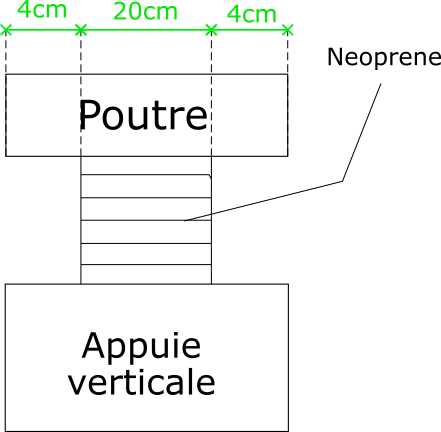
\includegraphics[width=0.7\linewidth]{figures/exo1/appiue-poutre-a}
	\end{minipage}
	\begin{minipage}{0.7\textwidth}
		
		Poutre sur appariel d'appuie :
		
		Dimension de l'appuie : $a = 4 + 20 + 4 = 28 ~\unit{cm}$
		
		largeur de la poutre : $b = 40 ~\unit{cm}$
	\end{minipage}

	\end{figure}
	
	
	\[ V_{\max} = 104040 ~\unit{N} < 0,237 \cdot 400 \cdot 280 \cdot 25 = 663600 ~\unit{N} \]
	
	
	
	\paragraph{Autre condition} :
	
	\[ A_{st_{adoptée}} = 13,44 ~\unit{cm^{2}} > 1,15 \cdot \dfrac{V_{\max}}{f_{e}} \]
	
	\[ 13,44 > 1,15\dfrac{104040}{400 \cdot 10^{2}} = 2.99 ~\unit{cm^{2}} \quad \text{ Condition vérifiée} \]
	
	
	\subsubsection{Armatures transversales}

	On peut Choisir l'espacement puis on determine la section ou le contraire.
	
	On choisie des armature transversale en cadre + étrier $HA6\rightarrow A_{t} = 1,13 ~\unit{cm^{2}}$
	
	4brins $A_{t} = HA6 = 1,13 ~\unit{cm^{2}}$
	
	
	\[ S_{t} \leq \min \left.\begin{cases}
		0,9 \cdot d \\
		40 ~\unit{cm}
	\end{cases}\right\}  = 40 ~\unit{cm} \]
	
	\[ S_{t} \leq \dfrac{A_{t} \cdot f_{e}}{0,4 \cdot b} = \dfrac{1,13 \cdot 400}{0,4 \cdot 25} = ????  \]
	
	\[ S_{t} \leq \dfrac{A_{t} \cdot 0,8 \cdot f_{e}}{(\tau_{u} - 0,3 \cdot f_{t28}) \cdot b} = \dfrac{1,13 \cdot 0,8 \cdot 400}{(0,562 - 0,3 \cdot 2,1) \cdot 25} =  - 21270,588 < 0 \]
	
	
	
	
	
	\section{Determination des armatures de la passerelle en BA (ELS)}
	
	
	\[ \overline{\sigma}_{bc} = 0,6 \cdot f_{c28} = 15 ~\unit{MPa} \]
	
	\[ \overline{\sigma}_{st} = 240 ~\unit{MPa} \]
	
	\subsection{Armatures de la dalle}
	
	\subsubsection{Calcul des charges}
	
	\begin{itemize}
		\item Revetement $\rightarrow 1000 ~\unit{N\per m^{2}} $
		\item Poids de la dalle $\rightarrow 1 \cdot 0,08 \cdot 25000 = 2000 ~\unit{N\per m^{2}} $ 
		\item Revetement + poids de la dalle = $ g = 3000 ~\unit{N\per m^{2}} $ 
		\item Surcharge d'exploitation $q = 4000 ~\unit{N\per m}$
	\end{itemize}
		
	
	\[ P_{ELS} = g + q  =  7000 ~\unit{kN\per m} \]
	
	
	\subsubsection{Calcul du moment}
	
	\[ M_{0} = \dfrac{7000 \cdot 2^{2}}{8} = 3500 ~\unit{Nm} \]
	


	\begin{center}
		
		\begin{tikzpicture}[scale=0.3]
			
			
			\draw[thick] (0,0) -- (2,0) -- ++(0,1.5) -- ++(5,0) -- ++(0,-1.5) -- ++(2,0);
			
			\draw[thick] (0,0) -- (0,4) -- ++(2,0) -- ++(0,-1.5) -- ++(5,0) -- ++(0,1.5) -- ++(2,0) -- ++(0,-4);
			
			\draw[<->, thick] (2,-1) -- ++(5,0) node[midway, above] {2 ~\unit{m}};
			
		\end{tikzpicture}
		
	\end{center}
	
	
	
	La dalle étant semi-encastrée sur les poutre latérale nous prenons :
	
	Sur appuie : $M_{a} = 0,4 \cdot M_{0} = 1400 ~\unit{Nm}$
	
	En travée : $M_{t} = 0,85 \cdot M_{0} = 2975 ~\unit{Nm}$
	
	\subsubsection{Calcul en travée}
	
	Pour la section en travée :
	
	Fissuration préjudiciable : $c = 2.5 ~\unit{cm}$
	
	
	\vspace{\baselineskip}
	
	La hauteur utile : $d = h - c = 8 - 2,5 = 5,5 ~\unit{cm}$
	
	
	\paragraph{Calcul de $\mu$}
	
	\[ \mu_{1} = \dfrac{M_{t}}{b \cdot d^{2} \cdot \overline{\sigma}_{st}} = \dfrac{2975 \cdot 10^{2}}{100 \cdot 5,5^{2} \cdot 240 \cdot 10^{2}} = 0,00409 \]
	
	Depuis les tableux par \underline{interpolation} on aura 
	
	\[ \mu_{1} \rightarrow \begin{cases}
		\beta_{1} = 0,8974 \\
		K_{1} = 33,7533
	\end{cases} \]
	
	
	\[ \sigma_{b} = \dfrac{\overline{\sigma}_{st}}{K_{1}} = \dfrac{240}{33,7533} = 7,1104 ~\unit{MPa} \]
	
	
	\[ \sigma_{b}  = 7,1104 ~\unit{MPa} \quad < \quad \overline{\sigma}_{b} = 15 ~\unit{MPa} \]
	
	\vspace{\baselineskip}
	
	
	\[ A_{st}^{ELS} = \dfrac{M_{t}}{\beta_{1} \cdot d \cdot \overline{\sigma}_{st}} = \dfrac{2975 \cdot 10^{2}}{0,8974 \cdot 5,5 \cdot 240 \cdot 10^{2}} \]
	
	\[ A_{st}^{ELS} = 2,511 ~\unit{cm^{2}} \]
	
	
	\begin{tcolorbox}[colback=gray!20, colframe=black, title=Remarque]
		Cette valeur étant supérieur a celle trouvée a l'ELU donc on va considérer celle a l'ELS
	\end{tcolorbox}
	
	
	\[ A_{st} = 2,511 ~\unit{cm^{2}} \]
	
	on prend 4HA10 = $3,14 ~\unit{cm^{2}}$ avec un espacement de 25cm.
	
	
	Les armatures de répartitions seront constitué de 4HA8 = $2,01 ~\unit{cm^{2}}$ pour 1ml. $\bigg(A_{r} = \dfrac{A_{st}}{4}\bigg) $
	
	
	Leur espacement sera de $25 ~\unit{cm} < 4 \cdot 8 = 32 ~\unit{cm}$
	
	
	\subsubsection{Calcul en appuie}
	
	\paragraph{Calcul de $\mu$}
	
	\[ \mu_{1} = \dfrac{M_{t}}{b \cdot d^{2} \cdot \overline{\sigma}_{st}} 
	=
	\dfrac{1400 \cdot 10^{2}}{100 \cdot 5,5^{2} \cdot 240 \cdot 10^{2}}
	= 0,00193 \rightarrow
	\begin{cases}
		\beta_{1} = 0,9265 \\
		K_{1} = 53,03
	\end{cases}
	\]
	
	
	\[ \sigma_{b} = \dfrac{\overline{\sigma}_{st}}{K_{1}} = \dfrac{240}{53,03} = 4,526 ~\unit{MPa} \]
	
	
	
	\[ \sigma_{b} = 4,526 ~\unit{MPa} < \overline{\sigma}_{b} = 15 ~\unit{MPa} \]
	
	\vspace{\baselineskip}
	
	\[ A_{st}^{ELS} = 1,145 ~\unit{cm^{2}} \]
	
	Comme $A_{st}^{ELS} > A_{st}^{ELU}$ on retiendra la valeur a l'ELS.
	
	\vspace{\baselineskip}
	
	On choisie 4HA10 = $3,14 ~\unit{cm^{2}}$ avec un espacement de 25cm.
	
	\vspace{\baselineskip}
	
	Les armatures de répartition : 4HA8 = $2,01 ~\unit{cm^{2}}$ avec un espacement de $25 ~\unit{cm} < 4 \cdot 8 = 32 ~\unit{cm}$
	
	
	
	\subsection{Armatures de la poutre}
	
	
	\begin{itemize}
		\item Garde-corps : $400 ~\unit{N}$
		\item Poids propre : $0,8 \cdot 0,25 \cdot 1 \cdot 25000 = 5000 ~\unit{N}$
		\item Reaction du Hourdis : $(3000 + 4000)\dfrac{2}{2} = 7000 ~\unit{N}$
	\end{itemize}
	
	Le tout pour 1ml.
	
	\[ P_{ELS} = 12400 ~\unit{N} \quad\text{pour 1ml} \]
	
	
	\subsubsection{Moment en travée}
	
	\[ M_{\max} = \dfrac{P_{ELS} \cdot l^{2}}{8} = \dfrac{12400 \cdot 12^{2}}{8} = 223200 ~\unit{Nm} \]
	
	\[ M_{\max} = 223200 ~\unit{Nm} \]
	
	\[ \overline{\sigma}_{s} = 240 ~\unit{MPa} \]
	
	
	
	\vspace{\baselineskip}
	
	
	\[ \mu_{1} = \dfrac{M_{\max}}{b \cdot d^{2} \cdot \overline{\sigma}_{s}} = \dfrac{223200 \cdot 10^{2}}{25 \cdot 74^{2} \cdot 240 \cdot 10^{2}} \]
	
	\[ \mu_{1} = 0,00679 \rightarrow \begin{cases}
		\beta_{1} = 0,8732 \\
		K_{1} = 24,9185
	\end{cases} \]
	
	
	\[ \sigma_{b} = \dfrac{\overline{\sigma}_{s}}{K_{1}} = \dfrac{240}{24,9185} = 9,6314 ~\unit{MPa} < \overline{\sigma}_{b} = 15 ~\unit{MPa} \]
	
	\[ A_{st} = \dfrac{M_{\max}^{^{appuie}}}{\beta_{1} \cdot d \cdot \overline{\sigma}_{s}} = \dfrac{223200 \cdot 10^{2}}{0,8732 \cdot 74 \cdot 240 \cdot 10^{2}} \]
	
	
	\[ A_{st}^{ELS} = 14,392 ~\unit{cm^{2}} > A_{st}^{ELU} = 13,44 ~\unit{cm^{2}} \]
	
	
	Alors les armature seront choisie avec la valeur a l'ELS.
	
	On choisie : 3HA20 + 3HA16 $= 15,45 ~\unit{cm^{2}}$ avec un espacement de 25cm.
	
	
	\begin{tcolorbox}[colback=gray!20, colframe=black, title=Remarque]
		Il s'agit d'une poutre de grande hauteur donc il faut prévoir des armatures de peau constituée de 3HA10 par face $(h > 50 ~\unit{cm})$ 
	\end{tcolorbox}
	
	
	
	
	
	\section{Plan de ferraillage}
	
	
	
	
	
	
	\begin{figure}[H]
		\centering
		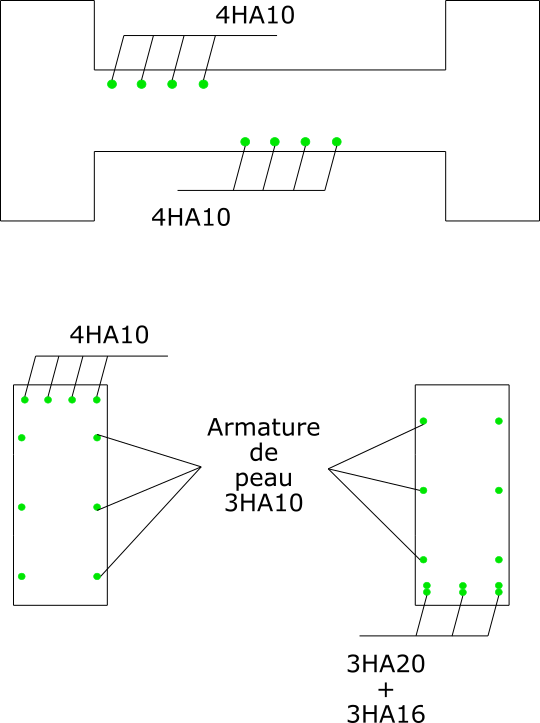
\includegraphics[width=0.7\linewidth]{figures/exo1/ferraillage}
		\caption{}
		\label{fig:ferraillage}
	\end{figure}
	
	
	
	
	
	
	
	
	
	
	
	
	
	
	
	
	
	
	
	
	
	
	
	
\end{document}